\begin{frame}[fragile]
  \frametitle{CUDA programming: shared memory, barrier}
\begin{itemize}
\item First let us implement straightforward matrix multiplication ({\color{mycolorcli}matrixMul0.cu})
  and then reimplement it using shared  memory ({\color{mycolorcli}matrixMul1.cu}) and compare performance between two GPU and CPU sequential implementations.
\item We define \mycode{Matrix} structure as follows:
{\color{mycolorcode}
\begin{verbatim}
typedef struct
{
  int width;
  int height;
  float * elements;
} Matrix;
\end{verbatim}
}
\item We allocate memory for matrices \mycode{A}, \mycode{B}, \mycode{C} on the host and device, generate random elements for \mycode{A} and \mycode{B} on the host and copy them to the device.
\end{itemize}
\end{frame}

\begin{frame}[fragile]
  \frametitle{CUDA programming: shared memory, barrier}
\begin{itemize}
\item To measure the timing for different kernels, we use cuda events:

{\color{mycolorcode}
\begin{verbatim}
cudaEvent_t start, stop;
cudaEventCreate(&start);
cudaEventCreate(&stop);
cudaEventRecord(start);

MatMulKernel<<<dimGrid, dimBlock>>>(d_A, d_B, d_C);

cudaEventRecord(stop);
cudaEventSynchronize(stop);
float milliseconds = 0;
cudaEventElapsedTime(&milliseconds, start, stop);
\end{verbatim}
}

\item In general, cuda events can be used to synchronize various threads.

\end{itemize}
\end{frame}

\begin{frame}[fragile]
  \frametitle{CUDA programming: shared memory, barrier}
\begin{itemize}
\item Notice that grids and blocks in CUDA can be 1-, 2-, 3-dimensional.
\item To multiply 2D matrices, it is natural to use 2D grids and blocks.
\item When calling a kernel, instead of 1D integers for grid and block sizes, 
  one can use 3D tuples of type \mycode{dim3}, in which by default, if not specified, all three components are set to 1:
{\color{mycolorcode}
\begin{verbatim}
dim3 dimBlock(BLOCK_SIZE, BLOCK_SIZE);
dim3 dimGrid(B.width/dimBlock.x, A.height/dimBlock.y);
...
MatMulKernel<<<dimGrid, dimBlock>>>(d_A, d_B, d_C);
\end{verbatim}
}
\end{itemize}
\end{frame}

\begin{frame}[fragile]
  \frametitle{CUDA programming: shared memory, barrier}
\begin{itemize}
\item In the first GPU implementation of matrix multiplication, we let each thread to 
  compute a separate entry of \mycode{C} matrix:
{\color{mycolorcode}
\begin{verbatim}
__global__ void MatMulKernel(Matrix A, Matrix B, Matrix C)
{
  float Cvalue = 0;
  int row = blockIdx.y * blockDim.y + threadIdx.y;
  int col = blockIdx.x * blockDim.x + threadIdx.x;
  for (int e = 0; e < A.width; ++e)
    Cvalue += A.elements[row * A.width + e] * 
              B.elements[e * B.width + col];
  C.elements[row * C.width + col] = Cvalue;
}
\end{verbatim}
}
\item Notice that \mycode{blockIdx}, \mycode{blockDim}, \mycode{threadIdx} are of type \mycode{dim3}
\end{itemize}
\end{frame}

\begin{frame}[fragile]
  \frametitle{CUDA programming: shared memory, barrier}
\begin{itemize}
\item We compare the performance of CUDA program with the performance of a single threaded straightforward matrix multiplication on CPU:
{\tiny
{\color{mycolorcode}
\begin{verbatim}
void sequential_cpu(Matrix A, Matrix B, Matrix C)
{
  for(int i = 0; i < C.height; ++i)
    {
      for(int j = 0; j < C.width; ++j)
        {
          C.elements[i*C.width + j] = 0;
          for(int ac = 0; ac < A.width; ++ac)
            {
              for(int br = 0; br < B.height; ++br)
                {
                  C.elements[i*C.width + j] += 
                    A.elements[i*A.width + ac] * 
                    B.elements[j + br*B.width];
                }
            }
        }
    }
}
\end{verbatim}
}
}
\item To multiply $160x240$ and $240x320$ matrices took $0.4$ ms with GPU implementation on K80 and $14320$ ms on a single Broadwell CPU core of \mycli{gpu2} partition. 
  Naive GPU implementation on a 4 year old K80 is $35800$ times faster!
\end{itemize}
\end{frame}

\begin{frame}[fragile]
  \frametitle{CUDA programming: shared memory, barrier}
\begin{itemize}
\item Notice: the first time the kernel runs on GPU in your program, it is slower than in subsequent times (0.6 ms vs 0.4 ms for this problem) due to some warming up overhead.
\item To take this into account, the kernel was called 5 times and the results are averaged over the last 4 measurements.
\item In this GPU implementation each element of \mycode{A} is read \mycode{B.width} times and each element of 
  \mycode{B} is read \mycode{A.height} times from global memory. 
\item Since global memory is slow, in ideal we want to read things from there only
  once and cache it in \mydef{shared memory} which is much faster. 
\item In ideal it would also be best to read data from global memory in a \mydef{coalesced} way to take advantage of automatic \mydef{caching} in L1, L2 caches:
  \begin{itemize}
    \item When you ask to read data at address \mycode{A} of size, say 4 bytes, instead hardware would read a \mydef{cacheline} of something like 32 of such elements and store them in fast but small cache.
    \item If the next address you read is available from cache, it is taken from there and global memory is not read
  \end{itemize}
\end{itemize}
\end{frame}


\begin{frame}[fragile]
  \frametitle{CUDA programming: shared memory, barrier}
\begin{itemize}
\item In the second implementation of matrix multiplication we shall divide each matrix into submatrices of $16x16$ size
\item Each thread block caches submatrix of \mycode{A} 
  and submatrix of \mycode{B} in shared memory before performing 
  a straightforward matrix multiplication of such submatrices.
\item As a result, each element of \mycode{A} is accessed {\color{mycolorcode}\verb|B.width/16|} 
  times and each element of \mycode{B} is accessed {\color{mycolorcode}\verb|A.height/16|} 
  times reducing the load on the global memory by a factor of $256$.
\end{itemize}
\end{frame}

\begin{frame}[fragile]
  \frametitle{CUDA programming: shared memory, barrier}
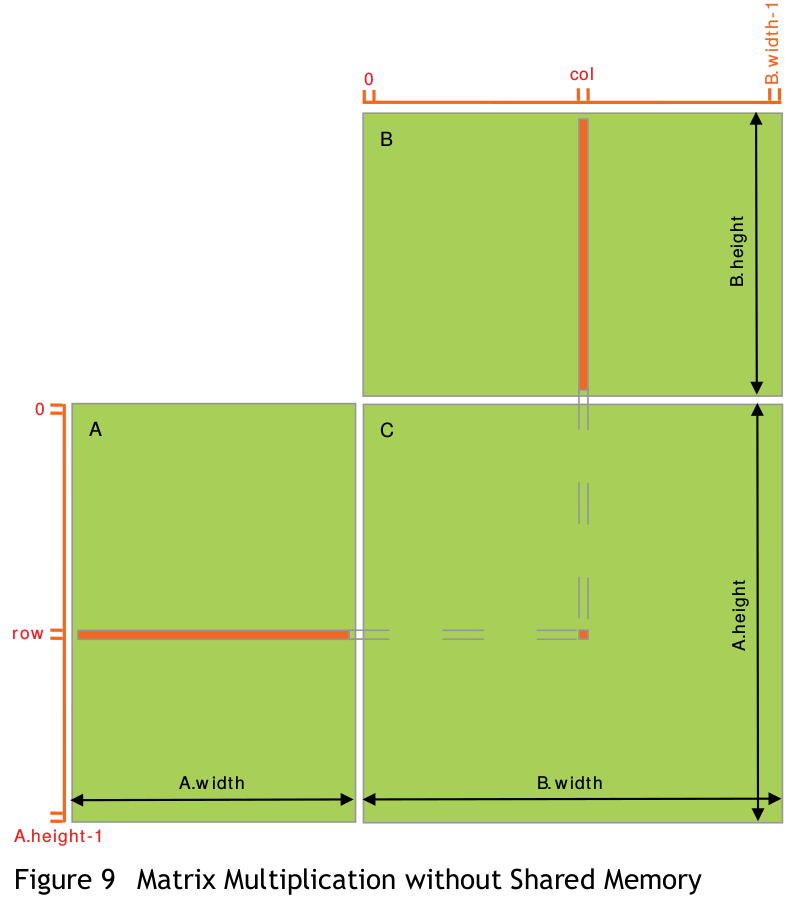
\includegraphics[width=5.5cm]{graphs/matMult1.png}
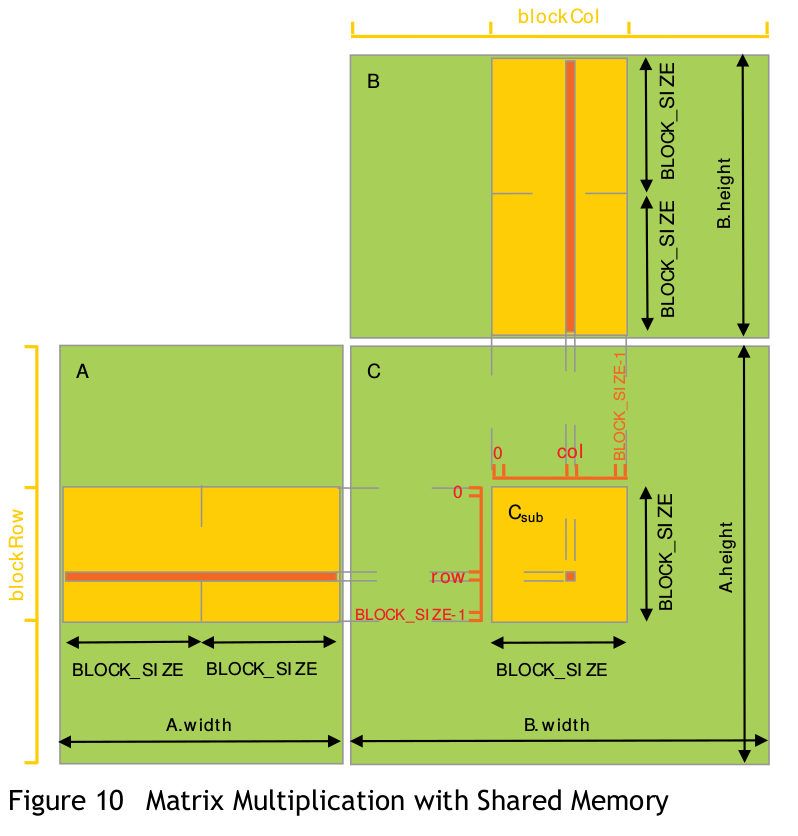
\includegraphics[width=5.5cm]{graphs/matMult2.png}
\end{frame}

\begin{frame}[fragile]
  \frametitle{CUDA programming: shared memory, barrier}
  \begin{itemize}
  \item To deal with submatrices, we need to modify the definition of the \mycode{Matrix} structure:
    {\color{mycolorcode}
      {\tiny
\begin{verbatim}
typedef struct
{
  int width;
  int height;
  int stride;
  float * elements;
} Matrix;
\end{verbatim}
      }
    }
  \item Here \mycode{width} refers to the width of the submatrix while \mycode{stride} refers to the width of the big matrix.
  \item Same structure can be used for the big matrix: 
    \begin{itemize}
    \item in that case \mycode{width = stride}.
    \end{itemize}
  \item The big matrix is subdivided into submatrices because you can store only so much in shared memory. For K80, it is up to 48kb.
  \end{itemize}
\end{frame}

\begin{frame}[fragile]
  \frametitle{CUDA programming: shared memory, barrier}
  \begin{itemize}
  \item We define several convenience device functions:
    \begin{itemize}
    \item to extract a submatrix in place:
      {\color{mycolorcode}
        {\tiny
\begin{verbatim}
__device__ Matrix GetSubMatrix(Matrix A, int row, int col)
{
  Matrix Asub;
  Asub.width = BLOCK_SIZE;
  Asub.height = BLOCK_SIZE;
  Asub.stride = A.stride;
  Asub.elements = &A.elements[A.stride * BLOCK_SIZE * row + 
                              BLOCK_SIZE * col];
  return Asub;
}
\end{verbatim}
      }
    }
    \item to get/set matrix element:
      {\color{mycolorcode}
        {\tiny
\begin{verbatim}
__device__ float GetElement(const Matrix A, int row, int col)
{
  return A.elements[row * A.stride + col];
}

__device__ void SetElement(Matrix A, int row, int col, float value)
{
  A.elements[row * A.stride + col] = value;
}
\end{verbatim}
      }
    }
    \end{itemize}
  \item Notice the above device functions are called from the GPU kernel that does the main job
  \end{itemize}
\end{frame}

\begin{frame}[fragile]
  \frametitle{CUDA programming: shared memory, barrier}
  \begin{itemize}
  \item Until compute capability 3.5, CUDA 5.0, only host could call a function that runs on GPU
  \item Now GPU functions can call GPU functions
  \item This feature is called \mydef{dynamic parallelism} and it  allows implementing, for example, recursive algorithms on GPU
  \item In the main kernel, each block computes a submatrix \mycode{Csub} by looping over submatrices \mycode{Asub} and \mycode{Bsub}
  \item Each submatrix is copied from the global memory into the shared memory
  \item All threads in a block wait on a \mydef{barrier} {\color{mycolorcode}\verb| __syncthreads()|} to make sure that all the necessary entries are loaded into shared memory
    before using them.
  \item Another barrier is inserted at the end of the loop iteration to make sure that all the threads in a block finished using shared memory before overwriting it with new submatrices
  \end{itemize}
\end{frame}

\begin{frame}[fragile]
  \frametitle{CUDA programming: shared memory, barrier}
{\tiny
{\color{mycolorcode}
\begin{verbatim}
__global__ void MatMulKernel(Matrix A, Matrix B, Matrix C)
{
  int blockRow = blockIdx.y;
  int blockCol = blockIdx.x;

  // Each thread block computes one sub-matrix Csub of C
  Matrix Csub = GetSubMatrix(C, blockRow, blockCol);

  // Each thread computes one element of Csub
  // by accumulating results into Cvalue
  float Cvalue = 0;

  int row = threadIdx.y;
  int col = threadIdx.x;

  // Loop over all the sub-matrices of A and B that are required to compute Csub
  // Multiply each pair of sub-matrices together
  // and accumulate the results
  for(int m = 0; m < (A.width/BLOCK_SIZE); ++m)
    {
      // Get sub-matrix Asub of A
      Matrix Asub = GetSubMatrix(A, blockRow, m);
      
      // Get sub-matrix Bsub of B
      Matrix Bsub = GetSubMatrix(B, m, blockCol);
\end{verbatim}
}
}
\end{frame}


\begin{frame}[fragile]
  \frametitle{CUDA programming: shared memory, barrier}
{\tiny
{\color{mycolorcode}
\begin{verbatim}
      // Shared memory used to store Asub and Bsub respectively
      __shared__ float As[BLOCK_SIZE][BLOCK_SIZE];
      __shared__ float Bs[BLOCK_SIZE][BLOCK_SIZE];

      // Load Asub and Bsub from device memory to shared memory
      // Each thread loads one element of each sub-matrix
      As[row][col] = GetElement(Asub, row, col);
      Bs[row][col] = GetElement(Bsub, row, col);

      // Synchronize to make sure the sub-matrices are loaded
      // before starting the computation

      __syncthreads();
      // Multiply Asub and Bsub together
      for(int e = 0; e < BLOCK_SIZE; ++e)
        {
          Cvalue += As[row][e] * Bs[e][col];
        }

      // Synchronize to make sure that the preceding
      // computation is done before load two new sub-matrices of A and B in the next
      // iteration
      __syncthreads();
    }
  // Write Csub to device memory
  // Each thread writes one element
  SetElement(Csub, row, col, Cvalue);
}

\end{verbatim}
}
}
\end{frame}


\begin{frame}[fragile]
  \frametitle{CUDA programming: shared memory, barrier}
\begin{itemize}
\item By using shared memory we further speed up the program by another factor of $2.5$: it now takes $0.16$ ms for the same matrices.
\item Trying to multiply big matrices on a single CPU core takes forever. 
\item Of course, on CPU one can also parallelize the program and take advantage of vectorization
\item There are 28 CPU cores on midway2 nodes
\item Vectorization might also give another factor of 16 or so
\item Still: to parallelize on CPU also requires some efforts (probably using OpenMP) and the expected performance gain would probably be 10-30 times worse than on K80.
\item Of course, this was just an excercise. To do linear algebra in your application, you should use libraries:
  \begin{itemize}
  \item on CPU: MKL, OpenBlas, Atlas, Plasma, Eigen, SuperLU...
  \item on GPU: cuBLAS, cuSPARSE, Magma...
  \end{itemize}
\end{itemize}
\end{frame}
